\documentclass[12pt]{article}
\usepackage{amsmath}
\usepackage{bm}
\usepackage{amssymb}
\usepackage{tikz}
\usepackage{tkz-euclide}
\usepackage{circuitikz}
\usepackage{pgfplots}
\usepackage[many]{tcolorbox}

\pgfplotsset{compat=1.18}

\newtcolorbox{boxA}{
colframe=white,
colback=white,
enhanced,
boxrule=1.5pt,
borderline = {0.75pt}{0pt}{dashed}
}

 
\tikzset{european}
\title{Nuclear Physics}
\author{Hertzberg, Joakim D.}
\date{\today}
\begin{document}

%END OF PREAMBLE

%title page
\begin{titlepage}
\maketitle
\begin{center}
\thispagestyle{empty}
\end{center}
\end{titlepage}

%table of contents
\tableofcontents

\newpage


%section 1: Particles
\section{Particles and their properties}
\subsection{The atomic mass unit}

The atomic mass unit (also \emph{AMU}) is defined as $1.66053907 10^{-27} \ Kg$. It has the unit \emph{u}.
It was defined such that the mass of a proton (and a neutron, which has the same mass) is $1u$.

\subsection{The electron}

The electron is an \emph{elementary particle}, which is a particle that has no building blocks, but is itself among the smallest possible building blocks.
The mass of an electron is $0.000548579909 \ u$, and it has a charge of $1.60217663 \times 10^{-19} \ C$, which is equal to the \emph{elementary charge} $e$.

\subsection{The proton}
The proton is a \emph{non-elementary} particle, which consists of \emph{quarks} which are elementary particles. It has a mass of $1.00727647 \ u$, and is positively charged by $+1 \ e$.

\subsection{The neutron}
The neutron is, as it's name implies, neutrally charged, meaning it has a charge of $0$, it has a mass of $1.008664915 \ u$.

\subsection{The positron}

The \emph{positron} is something which may also be encountered, and can easily be confused with the proton. It is significant to note that the positron is an \emph{elementary particle}, and is the anti-matter form of the \emph{electron}, so it has the same mass ($0.000548579909 \ u$), and a charge of $+1 \ e$.





%radiation

\section{Types of radiation}


%alpha-radiation
\subsection{$\bm{\alpha}$-radiation}
\emph{Alpha Radiation} or \emph{Alpha Decay} is when a particle releases another particle, a so-called \emph{$\alpha$-particle} as it decays.
$$^{A}_{Z}X \rightarrow \ \ ^{A-4}_{Z-2}X' + \ ^{4}_{2}\alpha$$

%Q-box
\begin{boxA}
	\textbf{\underline{What \emph{is} an $\bm{\alpha}$-particle?}} \bigbreak
	An alpha-particle looks exactly like a $He$-nucleus, that is, two protons \& 2 neutrons. Ignoring the amount of electrons, following is true: $$^{4}_{2}\alpha \ = \ ^{4}_{2}He$$
\end{boxA}

%beta-radiation
\subsection{$\bm{\beta}$-radiation}
\emph{Beta Radiation} or \emph{Beta Decay} is when a particle releases an electron and a neutrino as it decays, by a neutron splitting into an electron and a proton. 
\bigbreak
$$^{A}_{Z}X \rightarrow \ \ ^{A}_{Z+1}X' \ + \ ^{\ 0}_{-1}e \ + \ \bar{v}$$

%sidenote
\begin{boxA}
	\textbf{\underline{Sidenote:}} \bigbreak
Since elements release electrons as they decay, and gain a proton, the element itself changes to the next element over in the periodic table.
\end{boxA}

\subsection{$\bm{\gamma}$-radiation}

\emph{Gamma-radiation} or \emph{gamma decay} is when an 
excited particle de-excites and releases a photon, i.e. a $\gamma$-particle.
$$^{A}_{Z}X' \ \rightarrow \ ^{A}_{Z}X \ + \ ^0_0\gamma$$



%REACTIONS
\section{Nuclear Reactions}

%released energy
\subsection{Energy released}

In nuclear reactions, there is often a \emph{mass deficit} ($\Delta m$), which is then related to a certain energy which that mass converts into, $\Delta E$. Said energy is provided by Albert Einstein's famos equation: $$E = mc^2$$ \\
Which can be translated into: $$\Delta E = \Delta mc^2$$

%binding energy
\subsection{Binding Energy}
It has been found by scientists that there is more mass in an atom than the sum of all its \emph{nucleons}\footnote{A \emph{nucleon} is either a \emph{proton} or \emph{neutron}, i.e. a component of the nucleus}, this mass represents the \emph{binding energy}, which is the energy that is contained by the bonds which hold the neutrons particles together in the nucleus. This means that we can conclude following for an element $^{A}_{Z}X$: $$m_X - \Delta m \ = (Z)m_p + (A-Z)m_n$$
\bigbreak
NOTE: Binding energy is almost always the \emph{energy released} (see \textbf{\emph{3.1}})

\newpage

%example box
\begin{boxA}
	\textbf{\underline{Example:}}\bigbreak
	$^{54}Fe$ has a mass of $53.9396082 \ u$, a proton (with accompanying electron)
 has a mass of $1.0078250319 \ u$, and a neutron has a mass of $1.0086649 \ u$. \bigbreak

 \textbf{Q}: Find the binding energy of iron-54 \bigbreak

 Let $E_b$ be \emph{binding energy}

$$m_{Fe} - \Delta m \ = \ 53.9396 \ u \ = \ 26(m_p) + (54-26)(m_n)$$
$$53.9396082 - \Delta m \ = \ 26(1.0078250319) + 28(1.0086649)$$
$$53.9396082 - \Delta m \ = \ 52.42873823$$
$$\Delta m \ = \ 53.9396082 - 52.42873823$$
$$\Delta m \ = \ 1.51086997 \ u$$ \bigbreak
$$\because \left(\Delta E = \Delta m \times c^2 \right) \land \left(\Delta E \ = \ E_b \right)$$
$$E_b \ = \ \Delta m \times c^2$$
\begin{center}
Convert $m$ from $AMU$ to $Kg$. 
\end{center}
$$m = 1.51086997 \times 1.66053907 \times 10^{-17} \ = \ 2.50885861 \times 10^{-17}$$
$$E_b \ = \ 2.50885861 \times 10^{-17}(299 792 458)^2$$
$$E_b \ = \ 2.254849673 \ J$$
\end{boxA}

\newpage

%types of reactions
\subsection{Reaction Types}

\subsubsection{Transmutation}

It is possible to transmute one particle into the other by fusion. For example: $$^{14}_{\ 7}N \ + \ ^{4}_{2}He \ \rightarrow \ \ ^{17}_{\ 8}O \ + \ ^{1}_{1}H$$

\subsubsection{Fission}
A fission reaction is one where an atom is split into other atoms, this is usually done synthetically by bombarding the original atom with neutrons. $$^{A}_{Z}X \ + \ ^0_1n \ \rightarrow \ ^{A_1}_{Z_{1}}Y \ + \ ^{A-A_1}_{Z-Z_1-1}X' \ + \ 2\left(^{0}_{1}n \right)$$

\subsubsection{Fusion}
A fusion reaction is one where smaller nuclei react and create larger nuclei.
$$_{1}^2H \ + \ _{1}^3H \ \rightarrow \ ^4_2He \ + \ ^1_0n$$
Fusion reactions release very large amounts of energy, but 
they also require a lot of energy to be started. \bigbreak 

\begin{boxA}

	\textbf{\underline{Sidenote:}} \bigbreak

Fusion occurs in the sun, it may take place here due to the
extreme gravitational pressure exerted upon the core atoms
 by the rest of the star. The star then dies when the 
 internal pressure from fusion can no longer oppose the gravitation
 i.e. the core turns into $Fe$.

\end{boxA}

\newpage

\section{Half-life}

\subsection{What is half-life?}

Half life is \emph{the time it takes for an element to 
decay into half the element present}. \bigbreak

The equation for half-life is as follows: 
$$N_0\left(\frac{1}{2} \right)^\frac{t}{t_d}$$

\begin{center}
OR
\end{center}
$$e^{-\lambda t}$$ 

\begin{center}
Where $\lambda = \frac{1}{\tau}$ and $\tau=$ half-life
\end{center}
	\bigbreak

\begin{center}
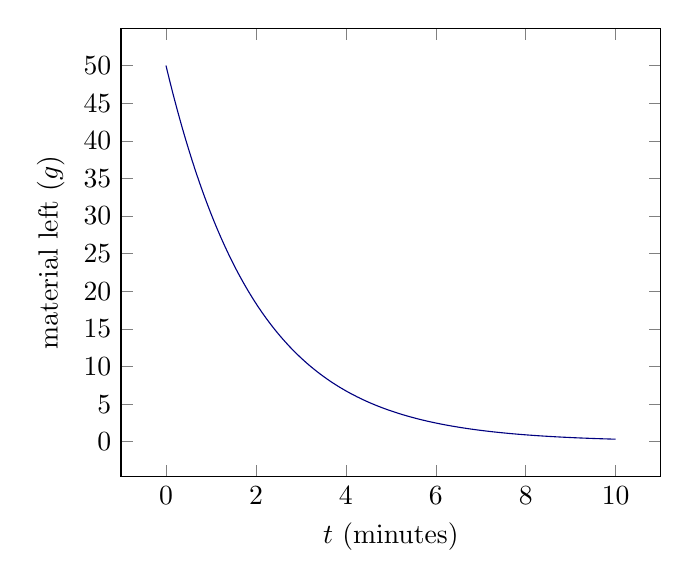
\begin{tikzpicture}
	\begin{axis}[
	samples=1000,
	xlabel = $t$ (minutes),
	ylabel = material left ($g$),
	xtick distance = 2,
	ytick distance = 5,
		]
	\addplot[color=blue!50!black, domain=0:10]{50*e^(-x/2))};
	\end{axis}
\end{tikzpicture}
\end{center}


\subsection{Activity}
\emph{Activity} is measured in $\frac{decays}{second}$, or 
\emph{Becquerelle} ($Bq$). \bigbreak
\end{document}
